\chapter{Problema 3}

\section{10594 - Data Flow}

En el laboratorio de IIUC, se requiere enviar una enorme cantidad de datos desde el servidor local hacia el terminal. La configuraci�n del laboratorio aun no esta lista. Requiere escribir un programa de ruteo para el mejor camino de datos. El problema es que todos los enlaces de la red tienen una capacidad fija y no puede fluir por ellos una cantidad mayor. Tambi�n toma una cierta cantidad de tiempo enviar una unidad de datos a trav�s del enlace. Para evitar las colisiones solo una unidad de datos puede viaja a la vez, por lo tanto, en un instante de tiempo no puede viajar en la red m�s de una unidad de datos en paralelo. Esto puede ser que consuma mucho tiempo pero asegura que no habr� colisiones. Cada nodo tiene suficiente capacidad de buffer de manera que los datos pueden ser temporalmente almacenados all�. La administraci�n de IIUC desea el menor tiempo posible para enviar todos los datos desde el servidor local hacia el final.

\begin{figure}[H]
\centering
\label{ejEnunciado_dataflow}
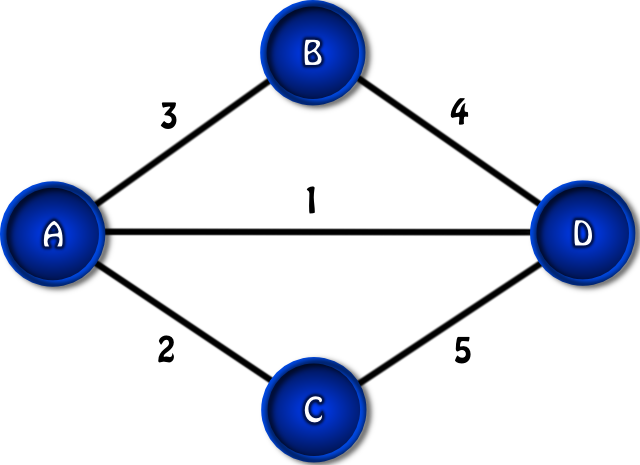
\includegraphics[scale=0.8]{./graficos/ej3/ejEnunciado.png}
\caption{Capacidad de los enlaces = 10}
\end{figure}

Por ejemplo, en esta red si alguien quiere enviar 20 unidades de datos desde A a D, enviar� 10 unidades de datos a trav�s del enlace AD y luego 10 unidades de datos a trav�s del enlace AB-BD, lo que tomar� 10+70=80 unidades de tiempo.

\textbf{Entrada:}

Cada input comienza con dos enteros positivos \textbf{N} ($2 \leq N \leq 100$), \textbf{M} ($1 \leq M \leq 5000$). En las siguientes l�neas siguen los links con su correspondiente tiempo de propagaci�n. Los links son bidireccionales y puede haber como m�ximo un link entre dos nodos de la red. En la siguiente l�nea habr� dos enteros positivos \textbf{D}, \textbf{K}, donde \textbf{D} es la cantidad de datos a ser transferida desde el 1er nodo hacia el \textbf{N}-�simo, y \textbf{K} es la capacidad de los enlaces. El input es terminado por EOF.

\textbf{Salida:}

Para cada test,  imprimir en una l�nea el m�nimo tiempo posible  para enviar todos los datos. Si no es posible enviar todos los datos, imprimir \"Impossible.\". El tiempo puede ser a lo sumo $10^{15}$.

\textbf{Url:}

\href{http://uva.onlinejudge.org/index.php?option=com_onlinejudge&Itemid=8&category=17&page=show_problem&problem=1535}{Problema de data flow}

\subsection{Modelo}

\subsection{Soluci�n}

\subsection{Detalles de implementaci�n}

\subsection{C�lculo de complejidad}